\section{Related Areas}
\label{sec:relwork}

%(related areas to ood: anomaly/novelty detection, open-set recog, etc.)

%There are several areas within the field of ML that are tangential to, and indeed have cross-pollinated with, OOD detection \cite{ghassemi2022comprehensive,cui2022out,shen2021towards}. \textit{Rejection} refers to the task of either accepting a given data sample as ``seen'' %during classification training 
%(analogous to ID data) or rejecting it as ``unseen'', typically with some associated cost \cite{cortes2016learning,geifman2017selective}. Works in this area parallel OOD detection in distinguishing between ID and OOD samples but focus more on optimizing for rejection costs \cite{cortes2016learning}. \textit{Anomaly detection} (or its close relative, \textit{novelty detection}) is the problem of detecting previously-unseen (i.e. anomalous or novel) data samples given some set of seen data \cite{tax2002one,liu2008isolation,andrews2016transfer}. Upon detection, the unseen data can then be either discarded, used to activate another behavior, or reserved for future training as a new task. Anomaly and novelty detection differ from OOD detection in that they do not consider the seen (ID) data for classification, instead treating the seen data as a whole solely for identifying unseen (OOD) data \cite{yang2021generalized}. OOD detection uses the classes inside of the ID data to better detect OOD data and often performs ID classification at the same time \cite{yang2022openood}. \textit{Open-set recognition} is a problem that somewhat overlaps with OOD detection. Methods in open-set recognition aim to simultaneously correctly classify known data encountered during training while also detecting unknown data at test-time \cite{scheirer2012toward,bendale2015towards,ge2017generative,neal2018open,scheirer2014probability}.
\gls{ood} detection as a domain of ML exists parallel to several other related fields, between which significant cross-pollination has occurred as ML has developed over time \cite{ghassemi2022comprehensive,cui2022out,shen2021towards}. The field of \textit{rejection} targets identifying and separating ``seen'' data samples (analogous to \gls{id} data) from ``unseen'' data samples, often using some cost to facilitate rejecting ``unseen'' samples during learning \cite{cortes2016learning,geifman2017selective}. Works in rejection are parallel to \gls{ood} detection but focus on optimizing for the aforementioned rejection cost instead of separating \gls{id} and \gls{ood} data \cite{cortes2016learning}. \textit{Anomaly detection} (or equivalently, \textit{novelty detection}) attempts to solve the problem of detecting data samples that have not been seen during training (i.e. anomalous or novel) \cite{tax2002one,liu2008isolation,andrews2016transfer}. Detected unseen data can be discarded or used in a variety of ways to facilitate additional procedures, such as future training as a new task. Anomaly and novelty detection differ only minutely from \gls{ood} detection. The primary difference is seen (\gls{id}) data and unseen (\gls{ood}) data are considered as whole collections in anomaly and novelty detection while \gls{ood} detection frequently leverages labels in \gls{id} data for detection \cite{yang2021generalized,yang2022openood}. In \textit{open-set recognition}, testing data is simultaneously classified and evaluated for similarity to known training data \cite{scheirer2012toward,bendale2015towards,ge2017generative,neal2018open}. The field overlaps with \gls{ood} detection.

%Other OOD detection-tangential fields in ML worth mentioning include \textit{uncertainty estimation} and \textit{causal representation}. The problem of uncertainty estimation in ML directly aims to quantify how uncertain a model is in a given data sample \cite{loquercio2020general,malinin2018predictive,malinin2019reverse}. %This can take the form of the complement to the maximum predicted class-distribution confidence produced by a model or some other metric estimating the model's recognition of the sample \cite{hendrycks2017baseline}. 
%This can take the form of an ML model's predicted confidence or some other metric estimating recognition of a sample \cite{hendrycks2017baseline}. Some methods in OOD detection make use of uncertainty estimation techniques to detect OOD samples at test-time \cite{hendrycks2017baseline,gal2016dropout,guo2017calibration}. %\textcolor{blue}{more could easily be added here if necessary} 
%Causal representation is a field that focuses on generating causal variables from observations that can then be used in causal graphs and reasoning \cite{scholkopf2021toward}. By using learned causal representations, models can infer whether encountered data samples are distributionally shifted (i.e. OOD) or not \cite{wang2022causal}. Another field similar to OOD detection is \textit{outlier exposure}, which uses ``outlier'' samples during training to explicitly learn what data should be considered as ``inliers'' (ID) or anomalies (OOD) \cite{hendrycks2018deep,yang2021generalized,chen2021atom,papadopoulos2021outlier}. This domain is not considered as directly comparable to OOD detection as it assumes access to OOD data during training, a violation of the OOD detection task definition. %\textcolor{blue}{TODO add outlier exposure here and emphasize it is not considered directly as OOD b/c they use OOD data}
Additional relevant fields tangential to \gls{ood} detection include \textit{uncertainty estimation} and \textit{causal representation}. ``Uncertainty'' in ML is a fundamental concept that quantifies the quality of a model's output, providing feedback on how uncertain a ML model is on a given data sample \cite{loquercio2020general,malinin2018predictive,malinin2019reverse}. With respect to \gls{ood} detection, this measure of uncertainty represents the model's confidence in the sample being \gls{ood} \cite{hendrycks2017baseline}. Uncertainty estimation underlies many state-of-the-art \gls{ood} detection methods \cite{hendrycks2017baseline,gal2016dropout,guo2017calibration}. Although less-directly related, causal representation nevertheless has shown value in \gls{ood} detection by learning causal representations and inferring if encountered data samples are \gls{ood} (i.e. distributionally shifted) \cite{scholkopf2021toward,wang2022causal}. \textit{Outlier exposure} (OE) is a prevalent tangential field that uses ``outlier'' data samples during training to learn differences between ``inlier'' (\gls{id}) and anomalous (\gls{ood}) samples \cite{hendrycks2018deep,yang2021generalized,chen2021atom,papadopoulos2021outlier,lioutlier,wei2024eat}. While OE solutions target the \gls{ood} detection problem, they are not directly comparable to non-OE \gls{ood} detection methods as they frequently assume access to \gls{ood} data during training. This violates the definition of the \gls{ood} detection task. However, recent work in OE has investigated generating synthetic outliers for training instead of assuming access to \gls{ood} data, a promising direction with great potential in realistic open-world applications \cite{gong2025out}. Of note is that \gls{ood} detection is not the same as \textit{\gls{ood} generalization}, which seeks to most effectively broadcast learned \gls{id} classes to potentially \gls{ood} testing data \cite{zangovercoming,li2023distilling,vogt2023robust}.

While the previous fields interleave with \gls{ood} detection, the field of \textit{continual learning} (CL) instead draws from \gls{ood} detection, utilizing it as a critical component in the conceptual and technical pipeline of CL. The task in CL is to incrementally learn a sequence of tasks \cite{thrun1995lifelong,hadsell2020embracing,chen2018lifelong}. It has been shown that the ability to understand when a new task has arrived fundamentally relies on \gls{ood} detection \cite{kim2022theoretical}. In the class-incremental learning (CIL) paradigm of CL, data is encountered over time but no indication is provided to the model regarding which task any given data sample belongs to. A CIL model must \emph{detect} if a data sample does not belong to previously encountered tasks - a problem that fits \gls{ood} detection \cite{kim2022multi,kim2023learnability}. CL stands as an example of how \gls{ood} detection plays an important role in open-world ML.

\section{OOD Detection Techniques}
\label{sec:relwork-ood}

\begin{figure}
 \centering
 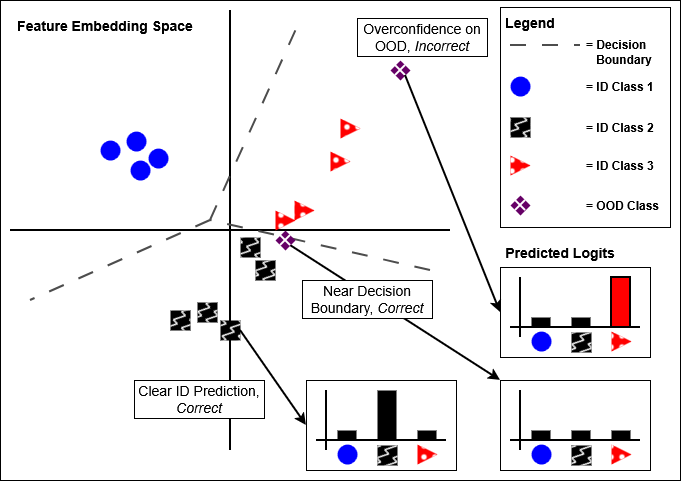
\includegraphics[width=0.9\linewidth]{figures/logits_describe}
  \caption{Example of the functionality of logits in detecting ID and OOD test samples. Overconfidence is a major issue with logits, incorrectly detecting the OOD sample in the upper right corner as ID.
  }
  \label{fig:relwork-logits_example}
\end{figure}

%(logit and confidence based methods, simple but subject to nn overconfidence and info loss)

%Initial attempts in OOD detection focused on leveraging ML model prediction outputs to measure model familiarity with encountered data samples. In what is often considered to be the seminal work in OOD detection, a neural network (NN) was trained to classify an ID dataset. Given a sample, the output logits of the NN %(resulting from processing the sample) 
%were converted to a prediction probability distribution using the softmax function %\textcolor{blue}{add a reference here, maybe say we will define it later and have a reference to the section} 
%and the maximum softmax probability (MSP) was treated as a measure of \emph{confidence} \cite{hendrycks2017baseline}. High MSP (confidence) values were characterized as a metric representing a low OOD score (i.e. more likely to be ID) while low MSP values were characterized as a high OOD score. This methodoloy was expanded upon in several directions, with some works directly using maximum logits as OOD scores \cite{hendrycks2019scaling}, normalizing the logits to reduce variance in predicted values \cite{wei2022mitigating}, or converting logits to energy values with less bias \cite{liu2020energy,wang2021energy}. Other research directions attempted to modify training procedures or adapt NN components to improve the utility of logits for OOD detection. The ODIN family of methods uses temperature scaling and input modification to estimate an OOD score based on how the logits change \cite{liang2017enhancing,hsu2020generalized}. Rectified Activations (ReAct) modulates NN intermediary layer outputs via clipping of activations, resulting in more distinguishable OOD logits \cite{sun2021react}. Generalize Entropy (GEN) modifies NN outputs using thresholded generalized entropy to reduce variance in predicted logits \cite{liu2023gen}. Further works leveraging logits for OOD detection have evaluated interpreting logits as density values \cite{abati2019latent,pidhorskyi2018generative,zong2018deep}, decomposed NN components for improved OOD detection with logits \cite{hsu2020generalized,huang2021mos,huang2021importance,devries2018learning}, utilized behaviors of NN weights to calibrate logits for OOD detection \cite{shama2019detecting,sun2022dice}, or investigated additional paradigms (prior networks \cite{malinin2019ensemble}, semantic representations \cite{shalev2018out}, classifier discrepancy \cite{yu2019unsupervised}) for improved logits-based OOD detection \cite{scheirer2012toward,smith1990extreme}. However, logits-based OOD detection methods are limited by two major factors. First, predicted logits inherently \emph{reduce the information} available in the model for identifying ID or OOD samples \cite{lee2018simple}. Second, NN models are known to be overconfident on predictions, regardless of if encountered samples are previously seen or unseen, significantly reducing their reliability for OOD detection \cite{nguyen2015deep,hendrycks2017baseline,wei2022mitigating,lee2018simple,sun2021react,paullada2021data}.
Preliminary exploration in \gls{ood} detection revolved around analyzing ML model predicted outputs for characterization of model familiarity with processed data samples \cite{yang2024generalized,lu2024recent} The seminal work in \gls{ood} detection trained an NN to classify \gls{id} data, then converted test data output logits into a probability distribution (using the softmax function). The maximum softmax probability (MSP) was treated as the measure of confidence in the sample being from the \gls{id} data distribution \cite{hendrycks2017baseline}. High MSP values were indicative of the sample being more likely \gls{id} (i.e. a \textit{low \gls{ood} score}) while low MSP values were indicative of the sample being more likely \gls{ood} (i.e. a \textit{high \gls{ood} score}). Future work innovated on this method in multiple ways. Some work elected to directly use logits for \gls{ood} scores \cite{hendrycks2019scaling}, others discovered the benefits of normalizing logits to reduce variance \cite{wei2022mitigating}, and promising advances have been made in converting model predictions from logits to energy measures with less bias \cite{liu2020energy,wang2021energy,chen2025dual}. Further investigations into the characterization of probabilistic classification models as energy models have leveraged architectural changes via Hopfield networks to more appropriately quantify energy-based \gls{ood} scores \cite{zhang2022out,hofmann2024energy,hofmannenergy,moriai2025rectified}. Alternative research directions instead have focused on improving model learning itself for \gls{ood} detection instead of limiting scoring to only the predicted outputs \cite{liu2024fast}. The family of ODIN \gls{ood} detection methods uses calibration (via temperature scaling) and modification of data inputs to estimate an \gls{ood} score based on changes in predictions \cite{liang2017enhancing,hsu2020generalized}. \gls{ood} detection from perturbing test inputs remains of interest, with recent investigations showing notable results \cite{chen2025leveraging}. Several works step further in this direction, using generative models and corruptions to estimate \gls{ood} scores \cite{lee2025hybood}. Rectified Activations (ReAct) clips the activations of NN intermediate layers, resulting in greater distinction between \gls{id} and \gls{ood} outputs \cite{sun2021react}. Generalized Entropy (GEN) uses thresholds on entropy functions of model outputs to reduce variance within \gls{id} and \gls{ood} outputs \cite{liu2023gen}. Adaptive Temperature Scaling (ATS) modulates temperature scaling in NN models to isolate \gls{id} predictions from \gls{ood} predictions \cite{krumpl2024ats}. Variational Rectified Activation (VRA) parameterizes ReAct and learns optimal clipping of activations to further optimize detection of \gls{ood} samples \cite{xu2024vra}. Adaptive Scaling (AdaScale) further builds on these ideas by identifying individual activation shifts between \gls{id} and \gls{ood} data, enhancing detection \cite{regmi2025adascale}. Other advances in logits-based \gls{ood} detection include interpreting predictions as density or entropy values \cite{abati2019latent,pidhorskyi2018generative,zong2018deep,yang2025eood}, decomposing NN components for improved logit characterization \cite{hsu2020generalized,huang2021mos,huang2021importance,devries2018learning,chen2023gaia,yu2023block,chen2024optimal}, and calibrating logits for \gls{ood} detection through analysis of NN weight trends during learning \cite{shama2019detecting,sun2022dice,canevaroadvancing,kalantransfer}. Additional logits-based paradigms include using prior networks \cite{malinin2019ensemble}, semantic representations \cite{shalev2018out}, ensembles \cite{yang2021ensemble,xu2024outofdistribution}, or optimizing classifier discrepancy \cite{yu2019unsupervised} for improved \gls{ood} detection \cite{scheirer2012toward,smith1990extreme}.

In modern \gls{ood} detection, it is recognized that logits-based methods are fundamentally limited by two major factors. First, logits \emph{reduce information quality} for \gls{ood} detection \cite{lee2018simple}. Second, it is well-recognized that NN classification models are \emph{overconfident on predictions}. That is, models are biased towards predicting higher confidences regardless of if the given data sample is \gls{id} or \gls{ood}. An example of overconfidence in \gls{ood} detection is shown in \ref{fig:relwork-logits_example}. The \gls{ood} sample in the upper right should be clearly \gls{ood} as it is far from any \gls{id} samples, but it is incorrectly considered \gls{id} due to overconfidence (represented as being clearly inside the \gls{id} class confidence region and far from any decision boundary). An additional non-trivial limitation is the assumption that prediction distributions learned by models are correct, while in practice this is not guaranteed \cite{liu2024rethinking,miao2024long}. This significantly reduces the capacity for models to perform \gls{ood} detection \cite{nguyen2015deep,hendrycks2017baseline,wei2022mitigating,lee2018simple,sun2021react,paullada2021data}.

%\textcolor{red}{TODO: add math and figures (can be ref to other works) here} % TODO overconfidence image maybe? LOW PRIO

%(self-supervised methods, powerful but very expensive, indirectly related to our ideas)

%A sub-direction of OOD detection methods attempts to resolve the overconfidence issue by exposing models to additional data and explicitly focusing model learning on discrimination of seen and unseen data samples \cite{hendrycks2019using,hu2020hrn,bergman2019classification,drozdova2024semi}. This sub-direction, commonly referred to as self-supervised methods, reduces prediction overconfidence by using self-supervised learning techniques to train OOD detection models on what is \emph{not} ID data \cite{hendrycks2019using}. A popular and powerful example of these methods in OOD detection is contrastive learning \cite{wu2018unsupervised,chen2020simple,qiu2021neural,chen2020simple}. Contrasting Shifted Instances (CSI) is a state-of-the-art contrastive learning method that uses rotated images and a contrastive loss to train the model to assign high predicted confidences to only the non-rotated image and low predicted confidences to all other (rotated) images \cite{tack2020csi}. CIDER uses a contraction loss and a dispersion loss to simultaneously coalesce ID data points within each class and separate ID class clusters in the learned feature space to ensure high predicted confidence only correlates with ID data \cite{ming2022exploit}. Several related directions use generative approaches to create examples of ``OOD'' data samples (derived purely from ID data), known as ``pseudo-OOD'' samples% for OOD detection training
%. Such methods use perturbed generated samples as pseudo-OOD examples \cite{oza2019c2ae,nalisnick2019deep}, adversarial training to directly teach models what is unfamiliar \cite{schlegl2019f,serra2019input}, or various class-informed generation \cite{wang2022cmg} and NN feature corruption \cite{du2022vos} approaches to generate and learn from pseudo-OOD samples. Other groups have explored a related direction, investigating the benefits of augmenting data for improving OOD detection models through exposure to data samples that are more generally representative of OOD distributions \cite{shorten2019survey,thulasidasan2019mixup,golan2018deep}. Data mixup uses data transformations and ID class mixing strategies to improve model OOD awareness \cite{thulasidasan2019mixup,yun2019cutmix,hendrycks2022pixmix,berthelot2019mixmatch}. Reconstruction \cite{denouden2018improving,zhou2022rethinking} and mixed image modeling \cite{li2023rethinking} leverage respective data augmentations to improve model familiarity with ID data and indirectly improve predictions for OOD detection. While self-supervised OOD detection methods have been found to be very powerful, they are expensive with respect to computational complexity and required resources. Furthermore, they do not resolve the issue of information reduction in logits-based OOD detection.
Attempts have been made to resolve the overconfidence issue in \gls{ood} detection through the well-studied domain of self-supervised methods. These attempts use additional data to focus model learning on discriminating between \gls{id} and \gls{ood} data \cite{hendrycks2019scaling,hu2020hrn,bergman2019classification}. By training models on what is \emph{not} \gls{id} data, overconfidence is reduced \cite{hendrycks2019scaling}. The predominant self-supervised \gls{ood} detection methods fall under the family of contrastive learning techniques \cite{wu2018unsupervised,chen2020simple,qiu2021neural}. Contrasting Shifted Instances (CSI) trains models using rotated images and a contrastive loss to concentrate predicted confidence on only the non-rotated images. This naturally distributes lower predicted confidence to all other non-rotated samples, simulating \gls{ood} samples during training and preparing the model for true \gls{ood} samples during testing \cite{tack2020csi}. The Compactness and DIspErsion Regularized framework (or just CIDER) learns to simultaneously coalesce \gls{id} data points within each class while separating \gls{id} data points between different classes, increasing predicted confidence for \gls{id} data \cite{ming2022exploit}. Another major self-supervised \gls{ood} detection direction generates ``pseudo-\gls{ood}'' samples that simulate \gls{ood} data using only \gls{id} data (as opposed to assuming access to the \gls{ood} data distribution, as in outlier exposure). These methods can use perturbed generated samples \cite{oza2019c2ae,nalisnick2019deep}, adversarial training \cite{schlegl2019f,serra2019input}, class-informed generation \cite{wang2022cmg}, or NN feature corruption \cite{du2022vos} to generate pseudo-\gls{ood} data. Other work has explored a tangential direction, using data augmentation to improve model learning of the \gls{id} data for greater recognition of \gls{id} test samples (and thus lower overconfidence in \gls{ood} test samples) \cite{shorten2019survey,thulasidasan2019mixup,golan2018deep}. Mixup uses data transformations and an \gls{id} class mixing strategy to improve \gls{id} data learning \cite{thulasidasan2019mixup,yun2019cutmix,hendrycks2022pixmix}. Reconstruction \cite{denouden2018improving,zhou2022rethinking} and mixed image modeling \cite{li2023rethinking} improve model familiarity with \gls{id} data using their respective data augmentations. Another direction in self-supervised \gls{ood} detection uses multiple models to promote learning of \gls{id} data and prediction consistency (e.g. between a teacher and a student) \cite{cai2022semi}. These techniques parallel the notion of mixture-of-experts, where multiple models are used to generate a prediction \cite{mu2025comprehensive,yu2024boosting}. Mixture-of-experts has also demonstrated impressive results in \gls{ood} detection \cite{lulearning,hogeweg2024cood}. \gls{ood} detection methods that rely on self-supervised methods have achieved impressive results, but they require significant data and computational resources. They also fail to solve the issue of information reduction provoked by logits-based \gls{ood} detection.

%\textcolor{red}{TODO: add math and figures (can be ref to other works) here} % TODO mixup image maybe? contrastive image maybe? LOW PRIO

%(distance-based methods, very competitive and use full information from model including features, nn components, etc.)

%Distance-based OOD detection resolves both issues present in logits-based OOD detection by using distances in some representative space defined by \emph{features} from the model. As the information for distance-based OOD detection is drawn from within the learned model, the dimensionality of the representative features is significantly larger than that of the predicted logits, allowing greater information representation for the processed data sample \cite{lee2018simple}. %Using distances to these features also helps eliminate overconfidence issues as feature distances are not conditional on a learned decision boundary determining model confidence in ID (or OOD) data \cite{} \textcolor{blue}{check wording/phrasing, maybe not make this claim}. 
%Mahalanobis Distance (MD) estimates distances between a data sample and approximate Gaussian distributions representing ID class data \cite{lee2018simple}. \textit{k}-Nearest Neighbor (KNN) uses the titular distance metric to measure the distance between a data sample and all ID data samples \cite{sun2022out}. Several other distance-based OOD detection ideas focused on using only important neuron outputs in NN models for feature generation and distance measurement \cite{olber2023detection,ahn2023line,dong2022neural}. Other techniques analyze use of different types of features in NN models \cite{abdelzad2019detecting,gunther2017toward}, features from different NN model architectures \cite{fort2021exploring}, and modulations of existing distance metrics \cite{ren2021simple,mendes2017nearest}. %\textcolor{blue}{can also add content here discussing how distance-based can theoretically be combined with other types of OOD detection e.g. self-supervised losses for improved feature learning, etc.} 
%Virtual-Logit Matching (ViM) uniquely combines features and logits via converting the model feature into a virtual logit before using it during logits-based scoring \cite{wang2022vim}. %A summary of previous OOD detection methods is presented in \textcolor{blue}{TODO - table}. 
%For distance-based OOD detection methods, greater distances indicate a higher OOD score (i.e. the sample is far from seen ID data) while lower distances indicate a lower OOD score. In addition to resolving the issue of information loss, distance-based OOD detection methods are advantageous because they use NN features which have been shown to be more resistant to overconfidence and thus more reliable for identifying OOD samples \cite{lee2018simple}. However, distance-based methods critically rely on discriminative features that are semantically representative of ID classes. While some success has been seen in combining self-supervised and distance-based OOD detection methods \cite{ming2022exploit,sehwag2021ssd}, learning effective features for consistent and reliable OOD detection remains a major challenge.
Both issues presented by logits-based \gls{ood} detection are solved with distance-based (or, equivalently, feature-based) \gls{ood} detection methods. By using distances in some representative space (typically defined by the embedded \emph{features} of a model), greater information is captured in the higher dimensionality (with respect to predicted logits) and overconfidence is mitigated through quantitative comparisons of embeddings instead of reduction into a probability distribution \cite{lee2018simple}. The primary representative distance-based \gls{ood} detection method, mahalanobis distance (MD), approximates Gaussian distributions around all \gls{id} class data for calculation of distances between test samples and \gls{id} classes. The minimum distance is used as a metric for the \gls{ood} score \cite{lee2018simple}. K-nearest neighbors (KNN) uses the titular unsupervised pipeline to measure the distance between \gls{id} data and potential \gls{ood} data samples \cite{sun2022out}. Class-Aware Relative Feature (CADRef) decouples relative features to measure distances with respect to \gls{id} classes \cite{ling2025cadref}. Discriminative Hyperspherical Embedding (DHE) uses normalization and regularization to improve \gls{id} class feature representation for greater \gls{ood} data separation \cite{zou2025provable}. Various other modulations of these distance metrics have been proposed for \gls{ood} detection \cite{ren2021simple,mendes2017nearest}. Other approaches to distance-based \gls{ood} detection focus on improving model learned features instead of improving on distance metrics \cite{kamkari2024geometric,guan2024exploiting,mirzaeiadversarially,li2024setar}. Deriving informed features from only important neuron outputs has been shown to improve distance-based \gls{ood} detection performance \cite{olber2023detection,ahn2023line,dong2022neural}. Principal Component Analysis (PCA) uses the named statistical technique to identify key components of model-learned features for more accurate distance measurements \cite{guan2023revisit,fang2024kernel}. Neural Collapse (NECO) identifies \gls{id}- and \gls{ood}-relevant components of features for \gls{ood} detection \cite{ammar2024neco,wupursuing}. Several works have proposed using ``typical features'', which are learned generalizable features for the training (i.e. \gls{id}) space, for \gls{ood} detection \cite{zhu2022boosting,he2024exploring}. Investigations into NN components and architectures have revealed multiple strategies for feature extraction in different models \cite{abdelzad2019detecting,gunther2017toward,yang2025oodd}. In particular, recent research has demonstrated that pre-trained foundation models can achieve state-of-the-art distance-based \gls{ood} detection performance using their general knowledge \cite{fort2021exploring}. A promising tangential direction to distance-based \gls{ood} detection combines feature-based distances and logits-based confidence. VIM converts model features into a virtual logit for an improved logits-based \gls{ood} score \cite{wang2022vim}.

While distance-based \gls{ood} detection methods have shown promising performance, they critically rely on discriminative features that are representative of \gls{id} classes. Some methods have observed success in using self-supervised techniques to improve the quality of features for distance-based \gls{ood} detection \cite{ming2022exploit,sehwag2021ssd}, but learning of effective discriminative features for generalizable \gls{ood} detection remains a significant problem in the field.

%\textcolor{red}{TODO: add math and figures (can be ref to other works) here} % TODO distance image maybe? LOW PRIO

%\textcolor{red}{TODO: (*** small table here summarizing prev ood works)} LOW PRIO

\begin{figure}
 \centering
 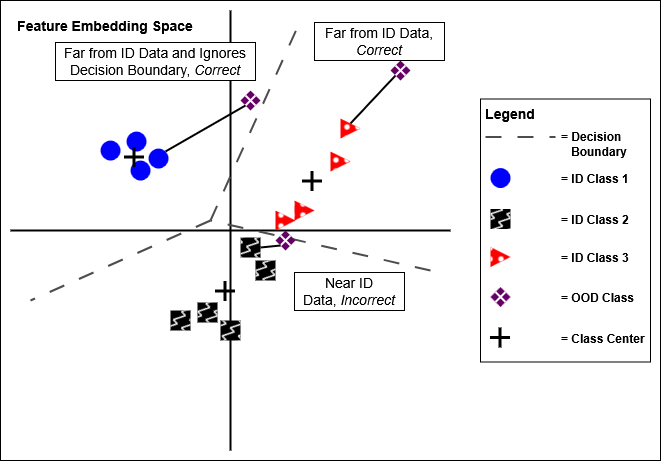
\includegraphics[width=0.9\linewidth]{figures/feats_describe}
  \caption{Example of the functionality of features in detecting ID and OOD test samples. Discriminative features are critical for OOD detection with features, leading to the issue with the lower OOD sample. Despite being near the decision boundary, it was detected as ID because it is close to ID data. Discriminative features would better separate the ID and OOD data in the feature space.
  }
  \label{fig:relwork-feats_example}
\end{figure}

The importance of features in \gls{ood} detection has become a major point of recent discussion in the field. A model's ability to learn \gls{id} class-representative discriminative features significantly influences its ability to distinguish \gls{id} testing data samples from \gls{ood} samples. This is illustrated in \ref{fig:relwork-feats_example}, where \gls{ood} data that lie near \gls{id} data in the feature space are incorrectly detected. Models that learn spurious features, which correlate to \gls{id} classes but do not contribute discriminative meaning, perform worse in \gls{ood} detection \cite{zhang2023openood,salehi2022unified}. Existing works have analyzed components of images, such as the backgrounds in images containing an object, to isolate sources of spurious features and develop mechanisms to prevent learning them \cite{ming2022exploit,neuhaus2023spurious}. The discussion of discriminative and spurious features is closely related to the well-known problem of near- and far-\gls{ood} detection. Specifically, the \gls{ood} detection problem is divided into two subsets according to difficulty in detecting the \gls{ood} samples. Far-\gls{ood} datasets are clearly separable from \gls{id} data, exhibiting severe covariate shift (differing domain from the overall \gls{id} distribution), severe semantic shift (differing features from the \gls{id} classes), or both. Near-\gls{ood} datasets overlap with the \gls{id} data distribution in some capacity, having little to no covariate or semantic shift \cite{yang2022openood,wang2023connecting,winkens2020contrastive,zhang2023openood}. The existence of near-\gls{ood} data is of critical importance in transitioning \gls{ood} detection from clinical environments to applications \cite{salehi2022unified,khazaie2022towards,wu2025out,zhang2021understanding,vaze2022generalized}. Several works have already begun to address the issue of adjusting \gls{ood} detection concepts and methods to realistic settings through adaptations such as improved outlier exposure \cite{azizmalayeri2022your} or robustness \cite{chen2020robust,meinke2022provably}. Despite these efforts, near-\gls{ood} detection remains a present issue in the field with many modern works neglecting to experiment on near-\gls{ood} datasets or struggling to outperform existing baselines \cite{gong2025out,ling2025cadref}. The near-\gls{ood} detection problem, and the related issue of learning discriminative features, exist as the next major challenge to both the field of \gls{ood} detection and the expansion of ML to open-world settings.

\section{Multi-View OOD Detection}
\label{sec:relwork-mvood}

%Multi-view classification \cite{seeland2021multi} has been studied by many researchers  \cite{su2015multi,zhao2023cddfuse} and used in numerous applications \cite{liu2019multi,zhan2023cfnet}. However, few works have leveraged foreground and background views of images \cite{geng2023foreground}.
%Recent progress has been oriented around the use of Transformer-based attention \citep{dosovitskiy2020image} layers \citep{zhao2023cddfuse,chen2021crossvit}. By using self-attention and cross-attention methods \citep{frank2021vision}, class-relevant features in data can be attended to both within and across views \citep{li2023mvhanet}. %Further performance gains were observed with further refinements to view feature fusion \citep{wang2024mutualformer} and alignment of learned features \citep{ke2024rethinking}. 
%Our work is different from cross-attention methods: (1) we leverage complementary information across three views using feature fusion in a novel hierarchical cross-attention and fusion architecture and (2) we uniquely apply this idea to foreground-background view data to improve OOD detection.
Multi-view classification is a field of ML that investigates the use of multiple different views of an images for a classification task. Each view is a distinct image derived from the original image and containing a subset of the features in the original image \cite{seeland2021multi}. Developments in the field have shown the benefits of multi-view learning in different architectures and across various applications \cite{su2015multi,zhao2023cddfuse,liu2019multi,zhan2023cfnet}. Recently, the prevalence of Transformer-based attention \cite{dosovitskiy2020image} has drawn the interest of the multi-view community. Studies have shown that models based on Transformers also benefit from multi-view learning, outperforming previous multi-view baselines (e.g. using convolutional NNs) \cite{zhao2023cddfuse,chen2021crossvit}. Innovations on self-attention and cross-attention methods \cite{frank2021vision} exploit the rich feature information across views \cite{li2023mvhanet} and enable fusion of view features into a more informative embedding for classification and other downstream tasks \cite{wang2024mutualformer,ke2024rethinking}. With respect to the choice of views, previous work primarily uses rudimentary transformations of the original image or different perspectives of the same object \cite{geng2023foreground}.

While multi-view classification has grown as a research field, there has been little-to-no work investigating the intersection between multi-view methods and \gls{ood} detection. Often, related works treat anomalous images (or components of images) as ``\gls{ood}'' and apply basic uncertainty estimation techniques to approximately detect these samples at test-time \cite{fernandez2023out,jung2022uncertainty}. Another work followed the related direction of augmenting images to separate \gls{id} images from anomalous images \cite{radford2021learning}.

%Little work has been done on multi-view OOD detection. One work used multi-view autoencoders to improve lesion detection in prostate cancer MRI images \cite{fernandez2023out}. \citet{jung2022uncertainty} improved OOD detection capabilities of multi-view Gaussian Processes. However, they do not consider deep NNs 
%and their views only vary the level of corruption noise injected into images. Another work uses CLIP \cite{radford2021learning} to identify ID-irrelevant nuisances to improve OOD detection but doesn't consider explicit image background separation or intelligent fusion of view features \cite{miyai2024locoop}. To our knowledge, no existing work has leveraged foreground-background views and feature fusion for OOD detection. An additional review of related work can be found in Appendix Sec. \ref{sec:suppmat-relwork}.
Image segmentation in multi-view contexts has only been sparsely explored. Within the field of \gls{ood} detection, several works have used foreground-segmented images for anomaly detection but they discard the background instead of utilizing it for additional features  \cite{tian2024foct,miyai2024locoop}. One solution used Vision Language Models and prompt learning to extract foregrounds, using \textit{both image and text} as input for few-shot \gls{ood} detection \cite{miyai2024locoop}. These approaches typically neglect full usage of all available image view features (e.g. backgrounds) or leverage other additional data modalities, rendering them incomparable to image-only or text-only \gls{ood} detection methods (which are the subject of this thesis). Another approach disentangles foregrounds and backgrounds in images but uses dense prediction instead of segmentation. It further applies the views to open-world classification instead of \gls{ood} detection \cite{ding2024improving}. Another typical problem exists at the frontier of segmented image-based, multi-view \gls{ood} detection research. Performance is generally poor compared previous single-view state-of-the-art \gls{ood} detection baseline methods. The problem of \gls{ood} detection using segmented images and multi-view methods remains open, with great potential.

\section{OOD Detection with Natural Language}

%In OOD detection, 
%\textit{confidence-based methods} use model logits to quantify confidence in a sample for evaluating its familiarity (i.e., ID or OOD) \cite{yang2024generalized,hendrycks2017baseline,wei2022mitigating,liu2020energy,sun2021react,liu2023gen,hofmannenergy}. Uncertainty estimation and augmented predictions have also been shown to improve logit quality for OOD detection \cite{thulasidasan2019mixup,liu2024fast,huang2021mos,sun2022dice,yu2023block,chen2024optimal,regmi2025adascale}.
%\textit{Self-supervised approaches} focus on learning better features for use in downstream OOD detection tasks \cite{hendrycks2019using}. Such methods include contrastive losses \cite{tack2020csi,ming2022exploit}, generative \cite{wang2022cmg,du2022vos} methods, or data augmentation \cite{zhang2024if,thulasidasan2019mixup, yun2019cutmix, hendrycks2022pixmix}. These methods have been explored in NLP and LLM-based OOD detection in varying capacities \cite{baran2023classical}.
%Domains related to OOD detection have been explored such as uncertainty quantification in LMs \cite{chen2024reconfidencing,ma2025estimating,xiong2023can,ye2024benchmarking}, OOD generalization \cite{wang2024can}, and quality assurance \cite{ouyang2025textual}, but have not been thoroughly applied specificlaly to the OOD detection problem \cite{zhou2023navigating}. 
%In natural language processing (NLP), OOD detection has also been studied \cite{lang2023survey,xu2024large}. Existing methods have shown fine-tuning on ID data to improve LLM OOD detection performance \cite{salimbeni2024beyond,zhang2024your,xu2022contrastive}. Other methods use model features or predicted logits and probabilities to quantify an OOD detection score \cite{lee2024ced,huang2024out,cao2024envisioning,baran2023classical}. However, all of these methods assume access to LLM components and training.
With the advent of large language models (LLMs), the field of natural language processing (NLP) has exploded in popularity. This has naturally nurtured an analogous growth in interest on the performance of such models when exposed to \gls{ood} samples \cite{baran2023classical,lang2023survey,xu2024large,yang2023out}. Related areas including uncertainty quantification \cite{chen2024reconfidencing,ma2025estimating,xiong2024can,ye2024benchmarking}, \gls{ood} generalization \cite{wang2024can}, and quality assurance \cite{ouyang2025textual} have attempted to establish the \gls{ood} detection problem in NLP \cite{zhou2023navigating}. Existing work on \gls{ood} detection in NLP have expanded other problems, such as the text classification task, to encompass identifying and classifying \gls{ood} test data \cite{zheng2020out,toth2024classification,garg2021towards}. More principled approaches consider quantifying the uncertainty in NLP-based methods and models \cite{da2024llm,xiong2024can,tian2023just}, including studying noise in NLP models and data \cite{al2021towards,chen2023automatic} and exposing models to synthetic \gls{ood} samples \cite{li2024conan,kim2023pseudo}.

With respect to LLMs, \gls{ood} detection has become a rapidly growing domain \cite{xu2025large,liu2024good,wang2024can,liu2024can,sali2025navigating,zaera2025efficient}. Initial work investigated fine-tuning to improve LLM characterization of the \gls{id} decision boundary and detection of \gls{ood} samples \cite{salimbeni2024beyond,zhang2024your,xu2022contrastive,hanparameter,kim2024investigation,wang2025chain,singh2025few,castillo2025intent}. Another direction of works instead focuses on improving and extracting LLM features or logits for \gls{ood} detection scoring \cite{lee2024ced,huang2024out,cao2024envisioning,baran2023classical,uppaal2023fine,tint2025prood}. In a set of works that draw from self-supervised learning, negative (i.e. synthetic alternative) classes or text domains were shown to be beneficial in augmenting LLMs for \gls{ood} detection \cite{huang2024out,luo2025semi}. Following from work in outlier exposure, success has likewise been observed in exposing LLMs to \gls{ood} data during training to improve \gls{id} and \gls{ood} separation at test time \cite{cao2024envisioning,park2023powerfulness,xu2023contrastive}. \gls{ood} detection in LLMs has also been considered as part of the design principles in many state-of-the-art foundation models. The inclusion of mixture-of-experts components in LLMs improves learning of discriminative \gls{id} knowledge, in turn improving uncertainty awareness during generation \cite{dai2024deepseekmoe,jiang2024mixtral}. Recent advances in agentic models have incited similar discussions on evaluating uncertainty awareness and improving \gls{ood} detection \cite{lee2025concept}. 

Of note is the recent focus of \gls{ood} detection on leveraging images and text, particularly in the form of Vision Language Models (VLMs) \cite{miyaigeneralized,lee2025harnessing,dai2023exploring,alnegheimish2025m}. Traditional methods, such as fine-tuning VLMs for \gls{ood} detection \cite{zeng2024local,xu2025overcoming}, have demonstrated clear effectiveness in solving the task. However, explorations into improving alignment between learned text and image embeddings suggests significantly greater depth in the multi-modal domain \cite{kim2025enhanced,zhang2025runa}. A greater interest in few-shot and zero-shot \gls{ood} detection has also developed recently, in which models must separate \gls{id} and \gls{ood} samples with either little-to-no \gls{id} training or no access to \gls{id} training samples at all \cite{madan2024revisiting,esmaeilpour2022zero}. 

\subsection{Prompting and OOD Detection}

One of the fundamental components in LLMs is the prompt, which contextualizes the task provided to the model and acts as the conditional distribution over which inference operates \cite{mei2025survey}. An expansive and rich history of investigations into prompts has resulted in a deep understanding on methods which improve LLM performance across a breadth of tasks. \textit{Reasoning} stands as a major prompting refinement (or equivalently, prompt engineering) method that encourages model refinement of knowledge \cite{munkhbat2025self,agarwal2023kitlm,zhou2022least,huang2023language,zhang2022automatic,shi2022language}. This can take multiple forms, including cognitive reasoning \cite{kramer2024unlocking} which aims to dissect LLM reasoning into a procedure of reasoning tools, or self-refinement \cite{madaan2023self,shinn2023reflexion,zhou2024isr} in which the LLM iterates over outputs until a consistent response is generated. Inclusion of examples within prompts, an example set of techniques being \gls{icl}, has been discovered to be extremely effective in many tasks \cite{dong2024survey}. Agentic prompting, resulting from the aforementioned increase in agentic LLM investigations, also shows promise in improving model efficacy \cite{yue2024fragrel,chen2022program}.

%Recently, a prompt-based method to OOD detection using LLMs was proposed. It does not have access to model features, logits, or fine-tuning. To our knowledge, \citep{wang2024beyond} is the sole study in this direction, using only prompts and detection of LLM response of ``unknown'' or a predicted intent to perform OOD detection. Specifically, a verbal prompt was used to provide the LLM with examples from ID classes and the input query before requesting the model to provide the corresponding ID class of the input or ``unknown'' if no ID class was relevant. The LLM output was parsed to identify if the correct class was generated for ID test samples or ``unknown'' was generated for OOD samples. We follow this direction and demonstrate that using more intelligent reasoning from the LLM, state-of-the-art prompt-only OOD detection can be achieved by converting existing OOD detection techniques into a prompt.
With respect to \gls{ood} detection, nearly all works in NLP- and LLM-based \gls{ood} detection assume access to model components (features and logits) or \gls{ood} data. The sparse domain of \textbf{prompt-only \gls{ood} detection} shows great promise in applications, functioning without unrealistic assumptions while improving model detection performance and increasing accessibility for users. Existing works are extraordinarily limited, with one work proposing the idea solely through generation of ``unknown'' or an \gls{id} class for detection \cite{wang2024beyond}. Prompt-only \gls{ood} detection exists as a task rich with potential for future innovation and application. In particular, the concept of \textit{alignment} \cite{yousef2020survey,wang2020measurement,bani2025hybrid,zaricna2015word,yang2019simple,chang2021deep,xylogiannopoulos2025power} has been thoroughly studied but has yet to be applied to \gls{ood} detection. Specifically, the notions of lexical alignment \cite{el2021xlent,dyer2013simple,srivastava2025measuring} and semantic alignment \cite{el2021xlent,thompson2020cultural} exhibit potential for use in \gls{ood} detection via prompting of LLM reasoning and generation of OOD scores.

%We evaluated their method both in the open-set classification setting and the OOD detection setting, and showed that in both cases the approach was suboptimal. Instead, we show that leveraging alignment with LLM reasoning and thesholding of OOD scores greatly improves performance and, interestingly, can even outperform feature- and logits-based OOD detection methods. We induce alignment through prompting of an LLM and find the utilization of both lexical alignment \citep{el2021xlent,dyer2013simple,srivastava2025measuring} and semantic alignment \citep{el2021xlent,thompson2020cultural} to be beneficial. Previous work on alignment manually defines alignment metrics and do not consider ICL. %, while we induce alignment in the generation of an LLM.
% new refs: to organize/add
% bani2025hybrid - alignment
% zaricna2015word - alignment
% yang2019simple - alignment
% yousef2020survey - alignment [survey]
% chang2021deep- alignment
% xylogiannopoulos2025power - alignment
% bhavana2024plagiarism - alignment (plagiarism)
% wang2020measurement - alignment [survey]
% sajid2025comparative - alignment (plagiarism)
% vrbanec2017struggle - alignment (plagiarism)
% chen2021empirical - MOCOv3
% oquab2023dinov2 - DINOv2
% caron2020unsupervised - SWAV

% TODO add below to nlp/llm section
%\vspace{2mm}
%\section{Related Work}
%OOD detection is a well-studied area with many effective techniques %solution to the open-world problem setting of ML 
%\citep{ghassemi2022comprehensive, zhang2023openood}.
%%OOD detection has been investigated from many different directions. 
%%Distance-based methods use a measure of distances, often in the model feature space, to detect OOD samples. Examples include Mahalanobis distance \cite{lee2018simple,ren2021simple}, %which uses covariance to estimate sample distance from ID data, 
%%non-linear space comparisons between samples \cite{sun2022out,regmi2024reweightood,ahn2023line}, and combined distance measurements between decomposed subspaces with logits-based confidence scores \cite{wang2022vim,ammar2024neco}.
%Logits-based methods use model predictions to estimate uncertainty in OOD samples \citep{hendrycks2019scaling}. Feature-based methods use measures of distance in the feature space, such as Mahalanobis distance \citep{lee2018simple,ren2021simple}, non-linear comparisons \citep{sun2022out,regmi2024reweightood}, and hybrid metrics \citep{wang2022vim,ammar2024neco}, to detect OOD samples.
%
%% llm
%% X - wang2024beyond (llm ood intent detect)
%% - liu2024good (llm ood detect)
%% X - wang2024can (icl ood generalization)
%% - liu2024can (ood detect from foundation models)
%% - dong2022survey (icl - survey)
%% X - lang2023survey (nlp ood detect - survey)
%% - zheng2020out (nlp ood detect - old, moderate citation count)
%% X - baran2023classical (ood detect* - classic methods w/ nlp models including llms)
%% X - chen2024reconfidencing (llm uncertainty - icl)
%% X - ma2025estimating (llm uncertainty)
%% X - xiong2023can (big llm uncertainty paper benchmark)
%% X - ye2024benchmarking (llm uncertainty benchmark)
%% X - lee2024ced (nlp ood detect - feats)
%%  + sample perturb is viable
%% - ouyang2025textual (nlp ood detect)
%% X - salimbeni2024beyond (llm ood detect - fine tuning)
%% X - zhang2024your (llm ood detect - fine tuning)
%% X - xu2024large (llm ood detect - survey)
%% X - huang2024out (llm ood detect - feats, vlm)
%% X - cao2024envisioning (llm ood detect - feats, vlm)
%% X - xu2022contrastive (llm ood detect - reqs separate trained model)
%% X - zhou2023navigating (llm uncertainty - it's unreliable)
%% *re-read and follow progression from nlp ood survey
%% singh2025few (need to train generative flow network, open-set classification)
%% castillo2025intent (fine-tuned LM + another LLM, open-set classification)
%% sali2025navigating (trained sentence transformer + another LLM, also open-set classification)
%% zaera2025efficient (trained LM, clustering required, fine-tuned LLM, also open-set classification)
%% tint2025prood (feature-based)
%% chow2025prompt (uses training for OOD detection)
%
%\textbf{Prompt-Only OOD Detection with LLMs.} 
%Recently, \citet{wang2024beyond} proposed a prompt-only ($C$+1)-classification method using LLMs, assuming no access to model features or logits. It addresses the OOD detection task tangentially but is the \textbf{only} previous work that considers prompt-only OOD detection.
%Specifically, it prompts an LLM with ID class examples and the input query before model output is parsed for either an ID class or ``unknown'' (OOD) if no ID class was relevant. 
%
%% The LLM output was parsed to identify if the correct class was generated for ID test samples or ``unknown'' was generated for OOD samples. 
%%To our knowledge, it is the sole study in this direction. However, our experiments show that our \sys outperforms this method. %We advance this direction by proposing to convert existing OOD detection methods into a prompt. % demonstrate that using more intelligent reasoning from the LLM, state-of-the-art prompt-only OOD detection can be achieved by 
%%It converts an existing OOD detection technique into a prompt.
%More related work is in Appendix Section 3.